\newpage
\subsection{SPI out}
This module is responsible for correct output of the data from the adder.




\subsubsection{Shift register}
The output consist of four sums, each containing 16 sum bits plus one carry output bit. This makes a total of 68 bits. To implement this we use a 68 bit shift register where each cell in the register contains one D flip-flop and one multiplexer. The multiplexer is used to switch between shifting and parallel load of the D flip-flop. In figure \ref{mux_dff} the schematic of a cell can be seen. 

\begin{figure}[H]
\centering
\captionsetup{justification=centering}
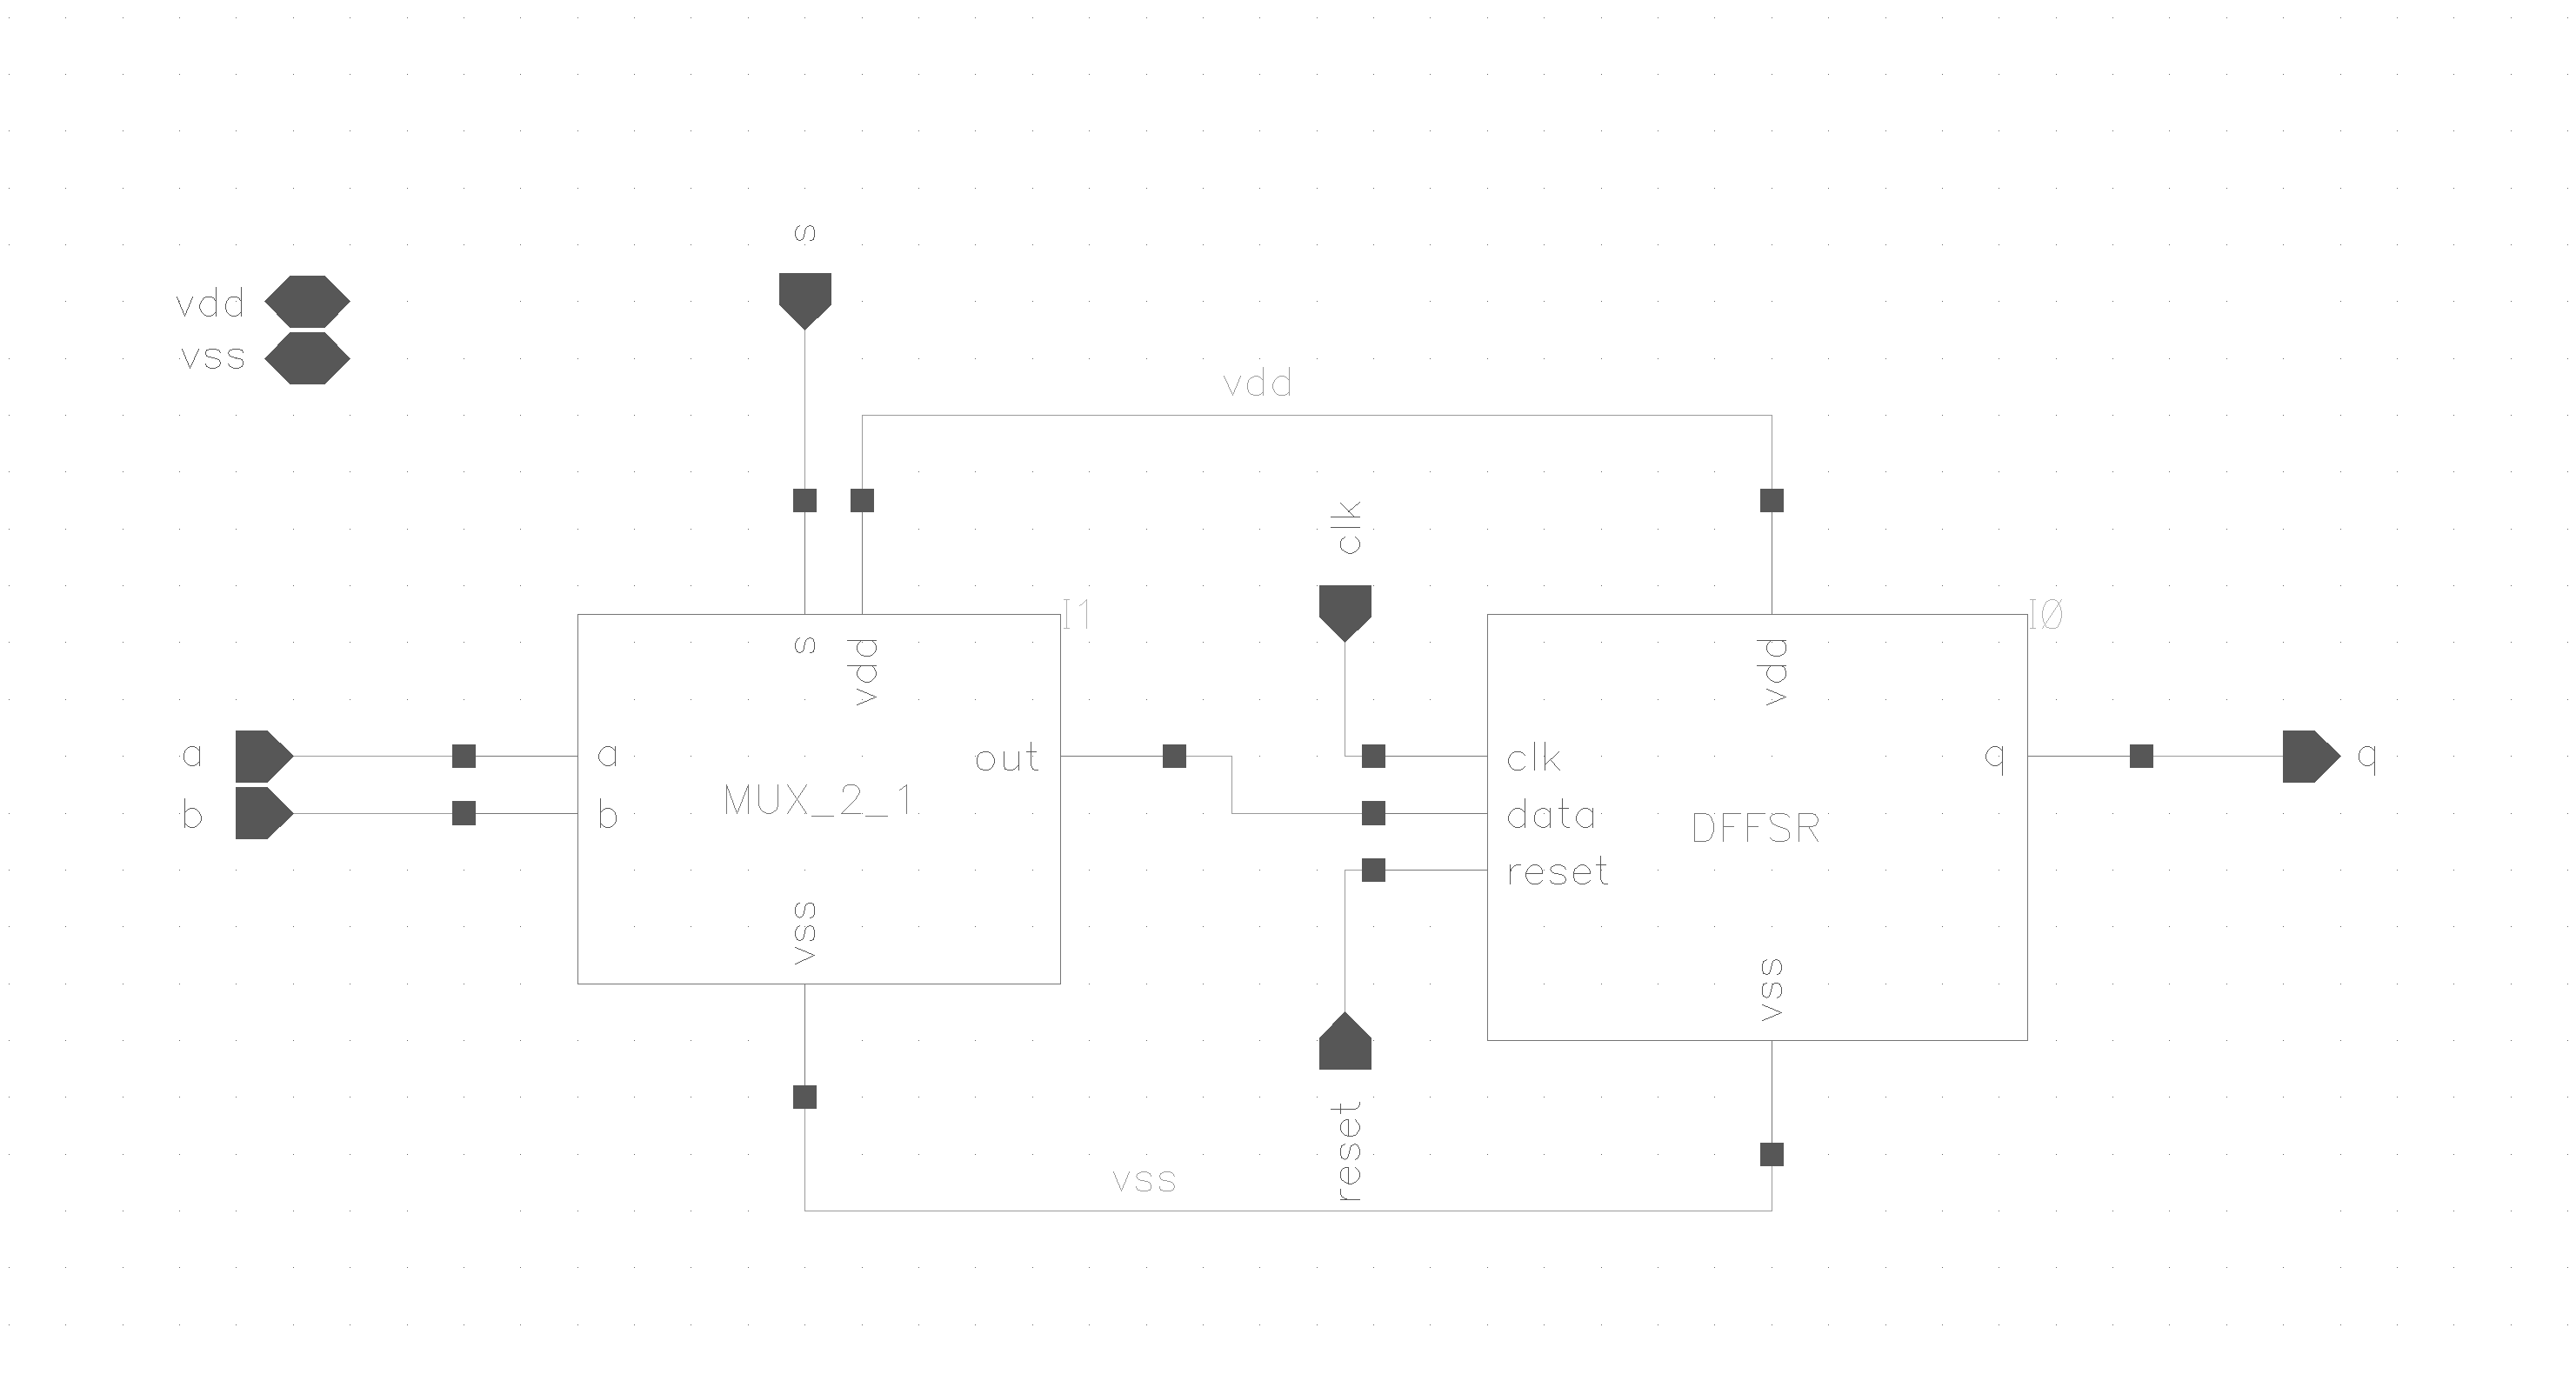
\includegraphics[scale=0.2]{../figures/mux_dffsr.png}
\caption{Shift register cell}
\label{mux_dff}
\end{figure}




\subsubsection{Control logic}
The control logic is needed to load the long shift register with the correct data. \\
As the adder is built in such a way that it executes all the four additions as fast as it can after the spi enable signal goes high, the output from one addition will only be available for one system clock cycle. This means that we need to quickly grab the data and put it in the correct place.\\ 
Our implementation uses a pulse generator, a 2-bit counter, a decoder to select what 17-bit part of the shift register to load, and some multiplexers to select if to clock the register on the spi clock or on the enable signals from the decoder. The pulse generator is triggered by the spi enable signal and creates a pulse that is four system clock cycles long. This to only allow the counter to increment four times, and also to clip the pulse from the last decoder output. As can be seen in \ref{spi_out1} the last output of the decoder is also feeded back to the enable of the counter through an inverter. This prevents a possible glitch that is generated when the counter starts over. The glitch would reload the section of the shift register containing the first sum. \\

\begin{figure}[H]
\centering
\captionsetup{justification=centering}
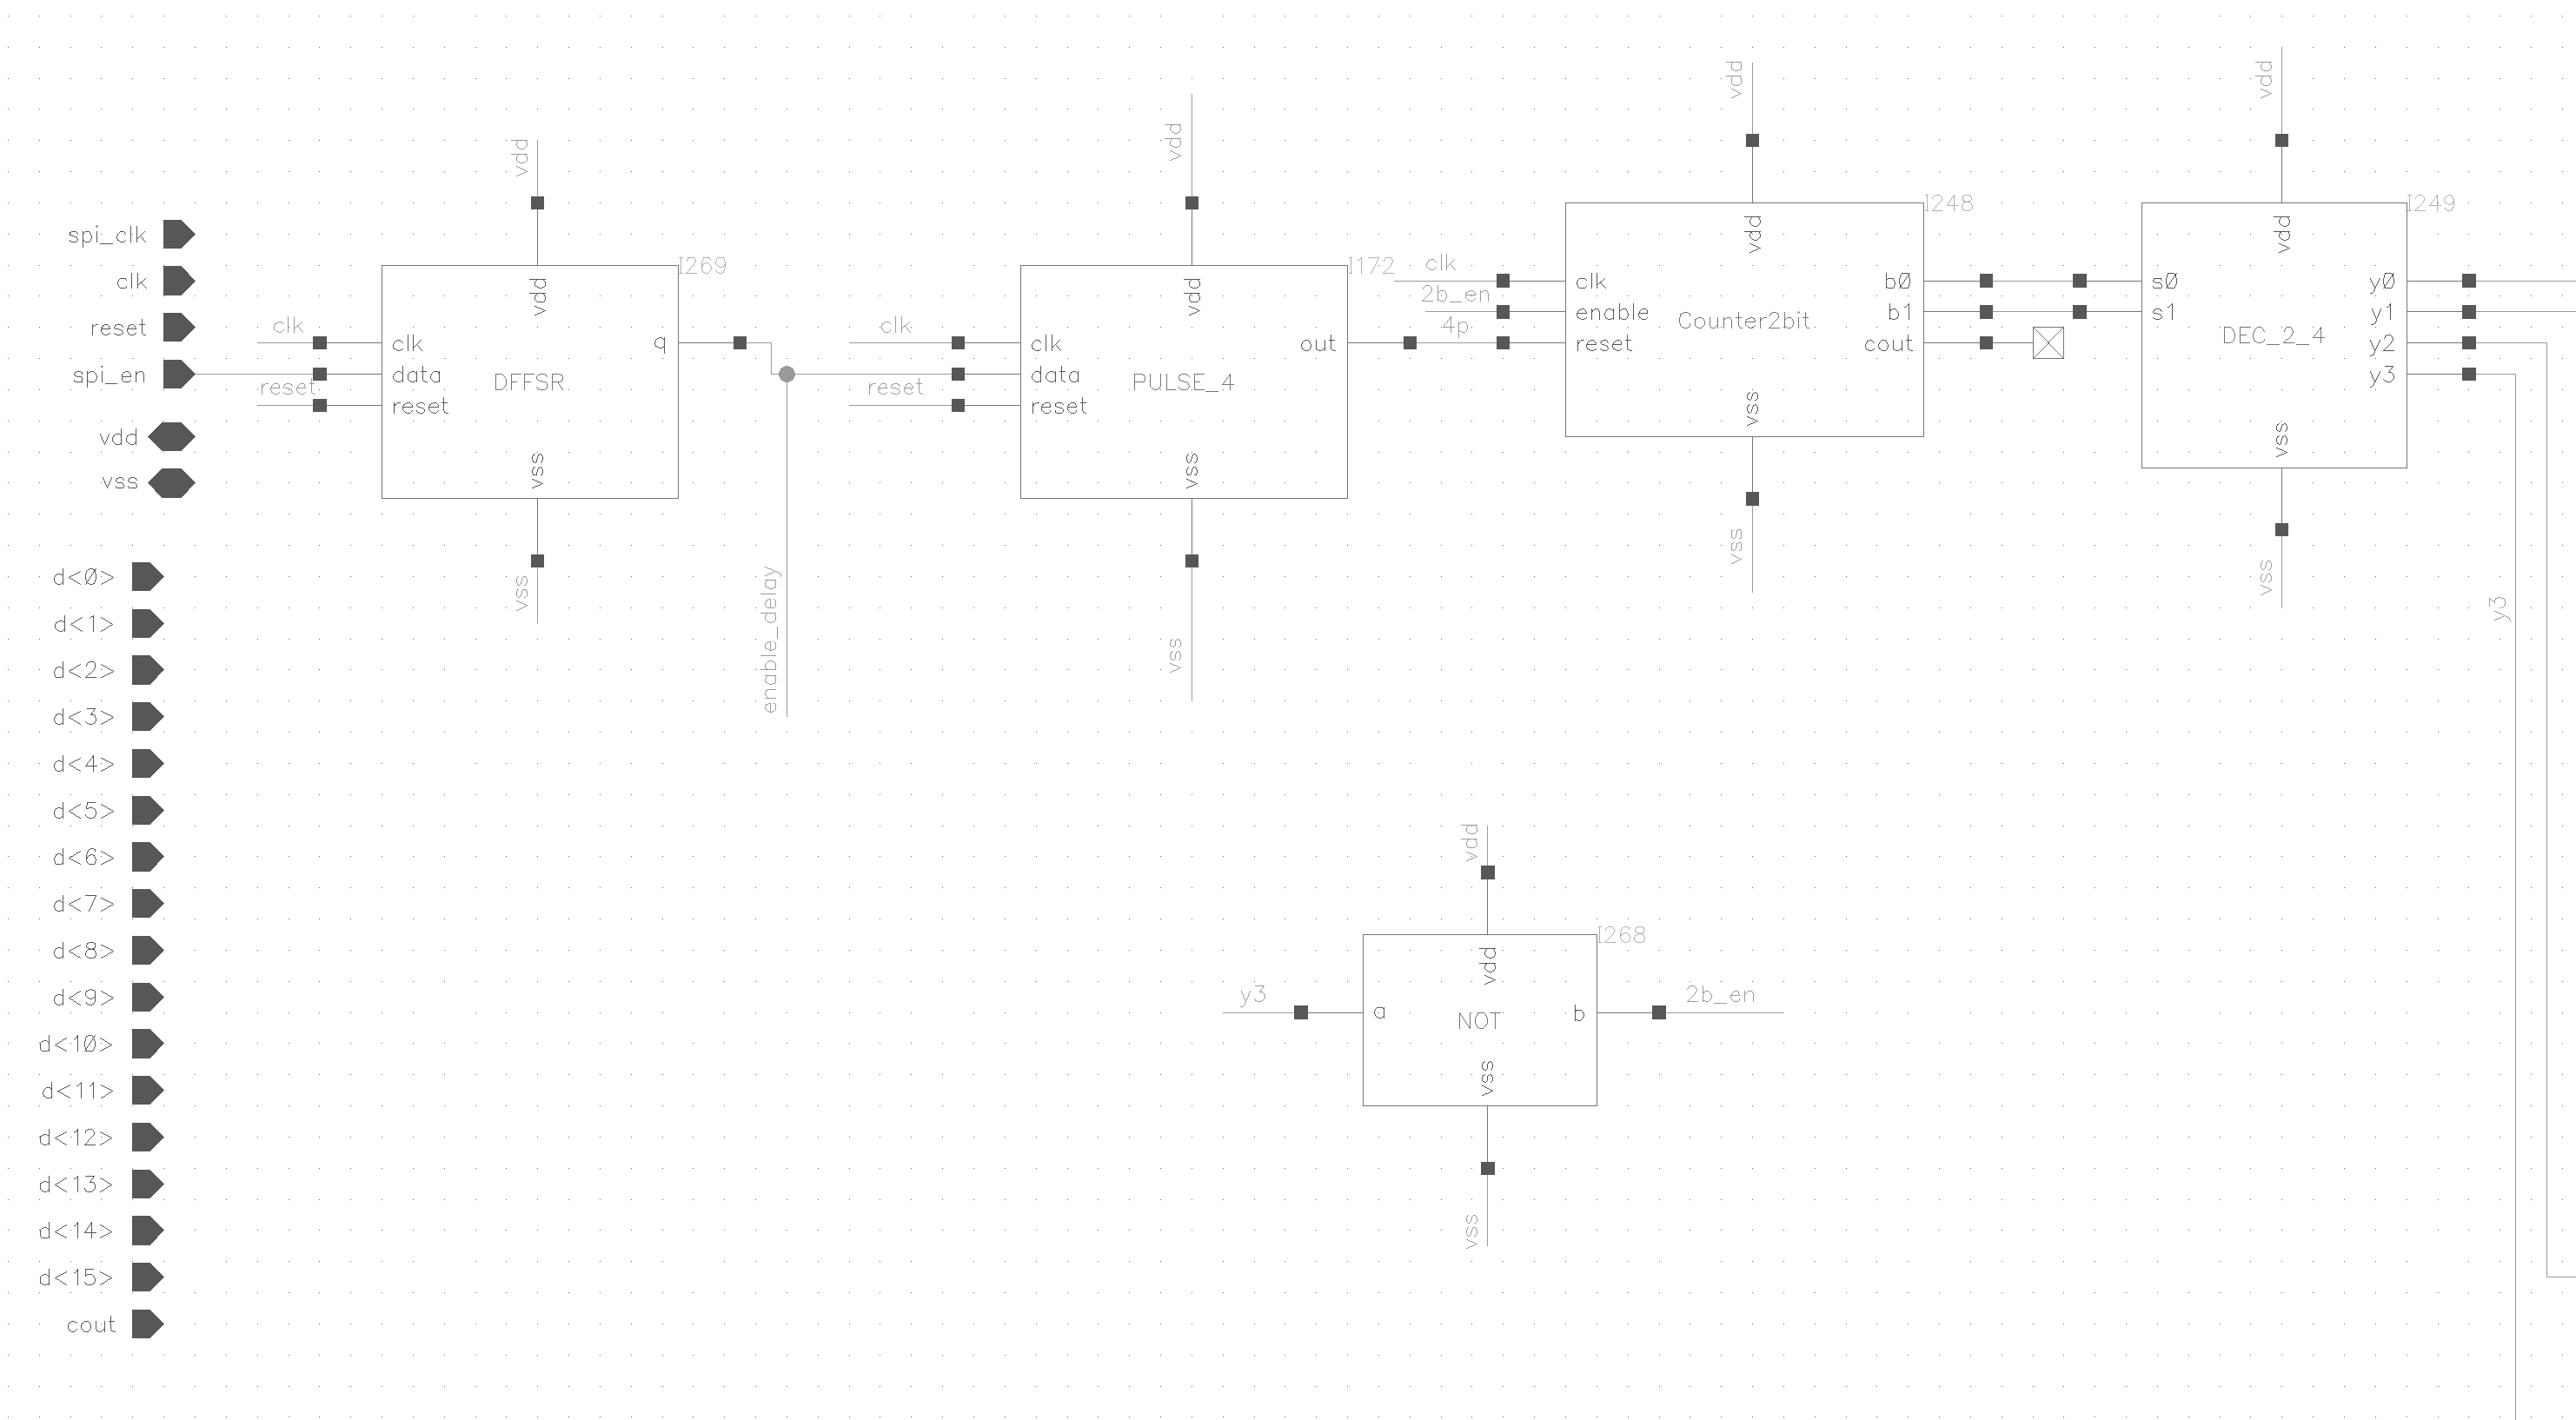
\includegraphics[scale=0.2]{../figures/spi_out1.png}
\caption{Control logic for spi output, first half}
\label{spi_out1}
\end{figure}

\begin{figure}[H]
\centering
\captionsetup{justification=centering}
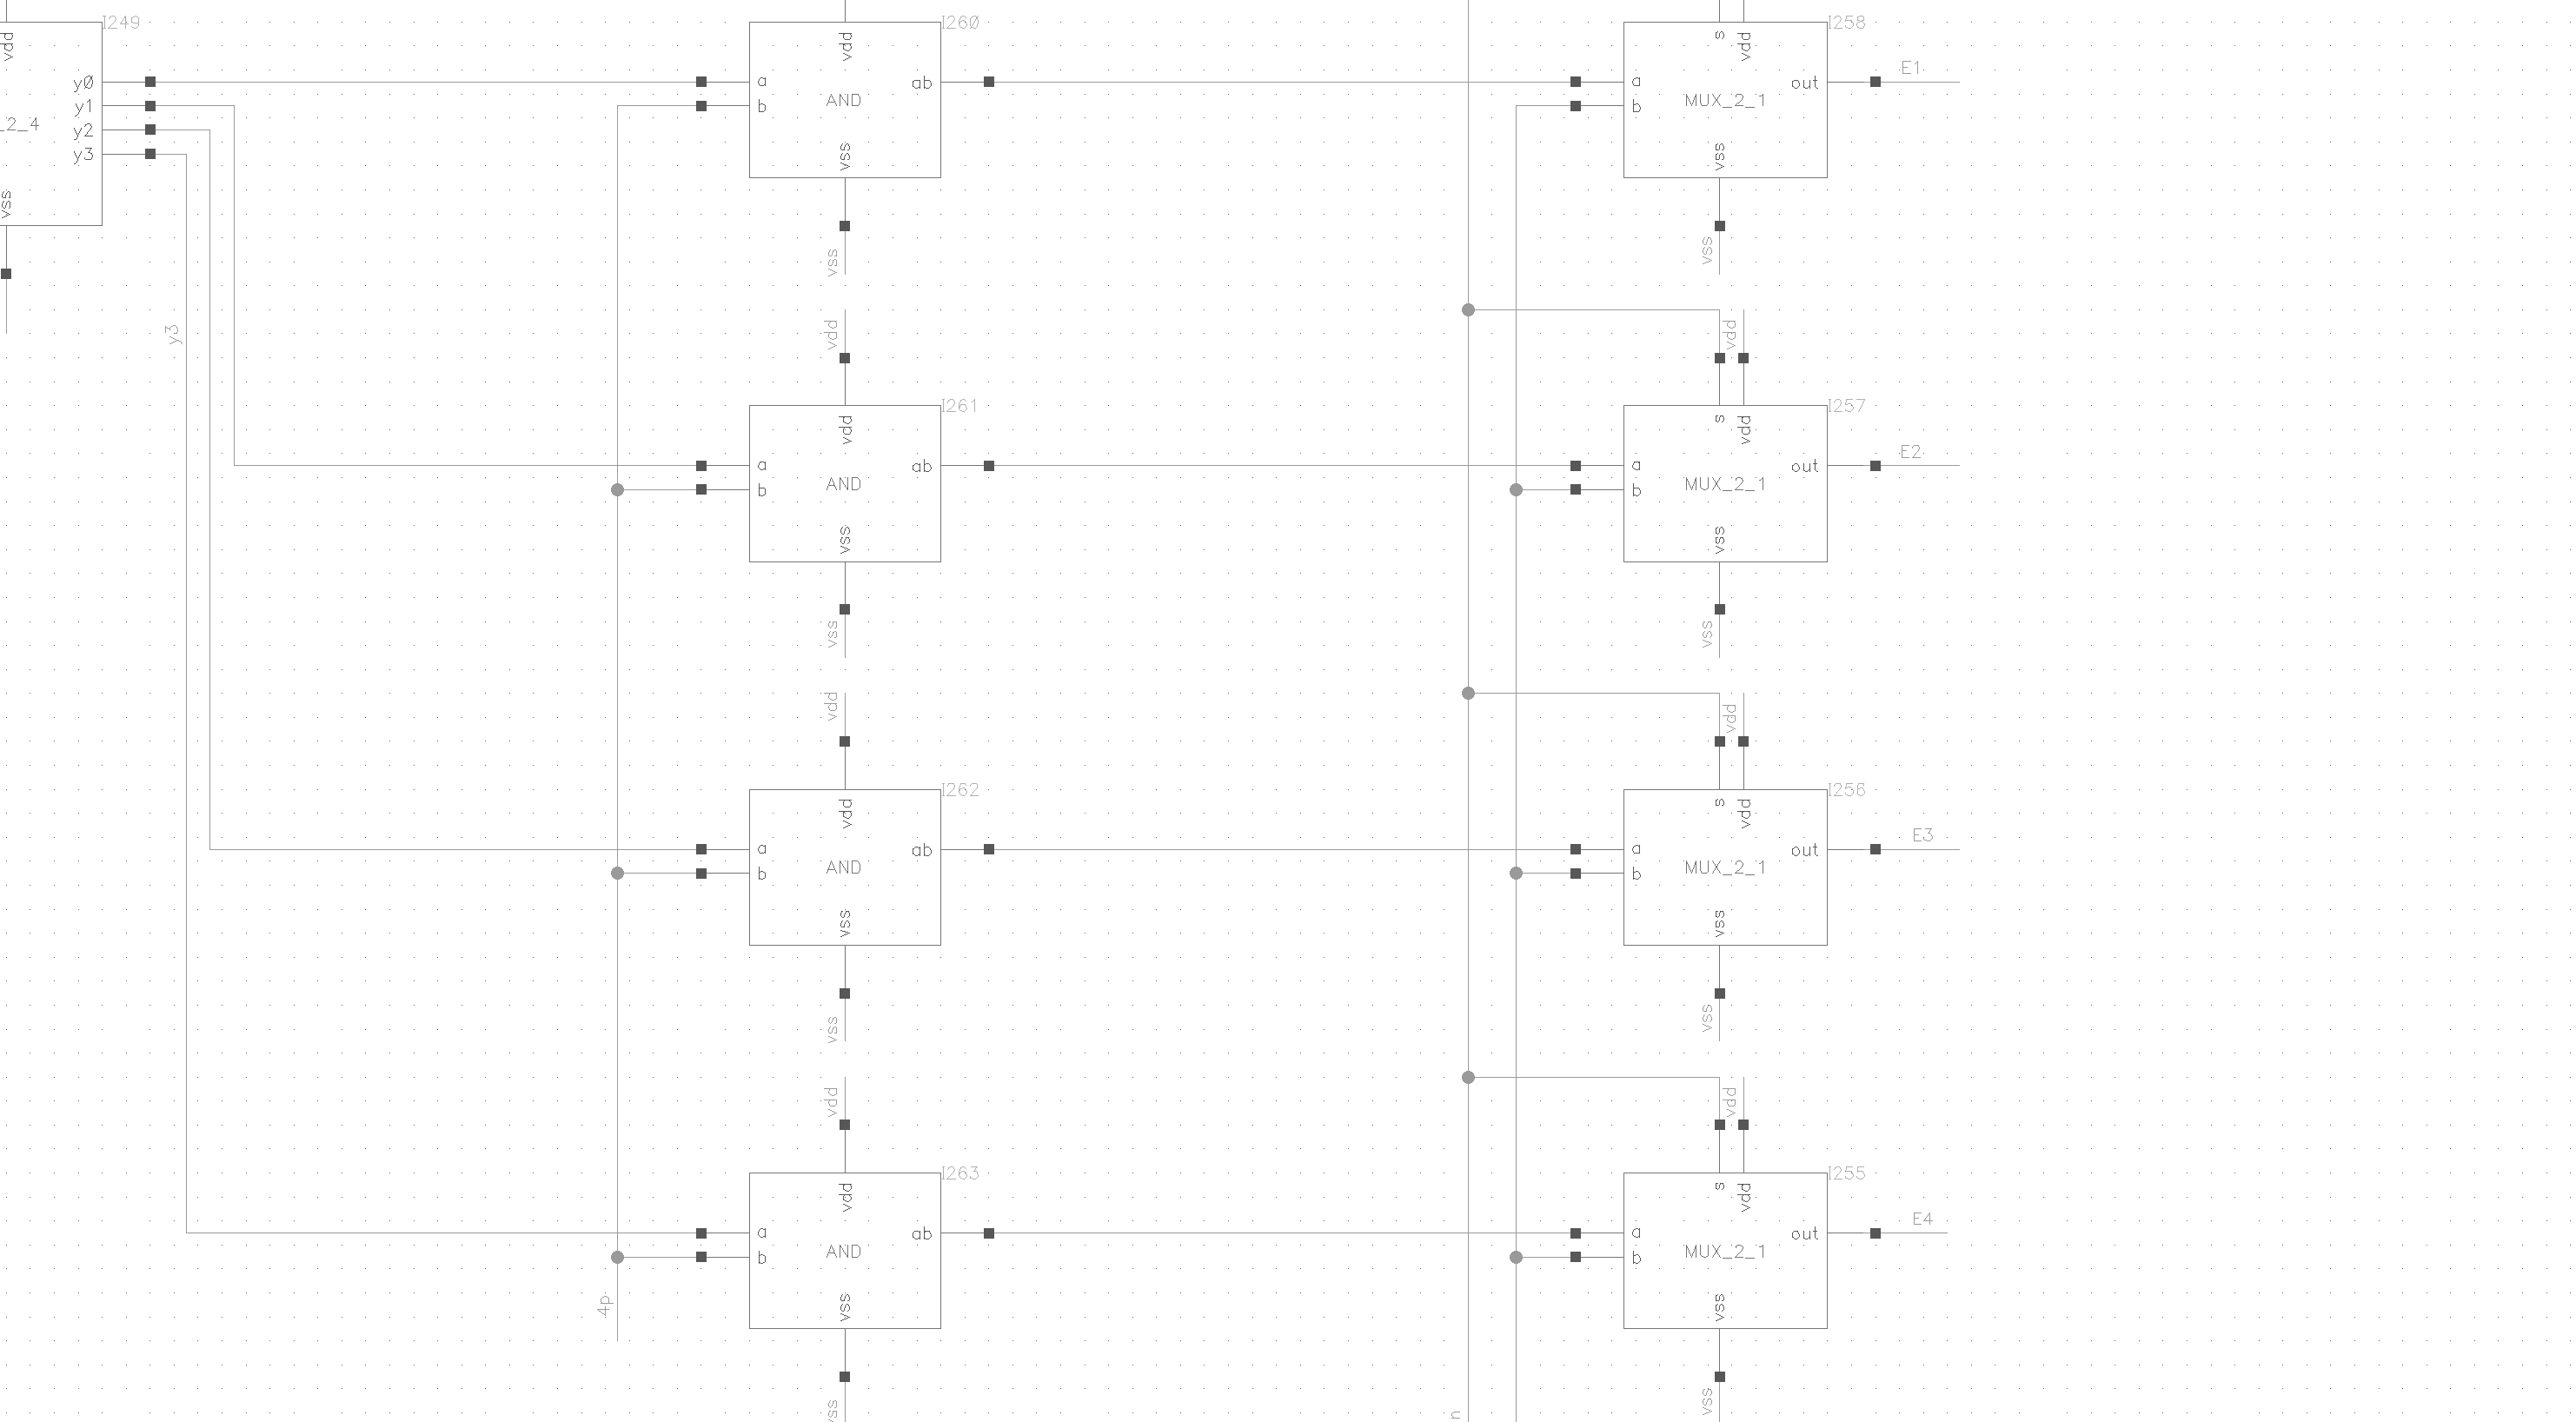
\includegraphics[scale=0.2]{../figures/spi_out2.png}
\caption{Control logic for spi output, second half}
\label{spi_out2}
\end{figure}

\subsubsection{Protocol}
This unit outputs the data with most significant bit first, in this case the carry output. To not use 
